%!TEX root = ../dokumentation.tex

% Deckblatt für Studienarbeiten

\begin{titlepage}
\newgeometry{left=2.5cm,right=2.5cm,top=2cm,bottom=2.5cm}

\centering
\begin{figure}[t]
    \begin{minipage}[]{0.49\textwidth}
        \flushleft
        
\includegraphics[width=2.5cm]{images/essential/firmenlogo.png}
    \end{minipage}
    \begin{minipage}[]{0.49\textwidth}
        \flushright
        
\includegraphics[width=3.9cm]{images/essential/dhbw.png}
    \end{minipage}
\end{figure}

\enlargethispage{20mm}

\begin{center}
	\vspace*{6mm}	{\arbeit}\\
	\doublespacing
	\vspace*{12mm}	{\LARGE\textbf{{\titel}}}\\
	\onehalfspacing
	%\vspace*{12mm}	%\langdeckblattabschlusshinleitung\\
	%\vspace*{3mm}		{\textbf \abschluss}\\
	%\vspace*{12mm}	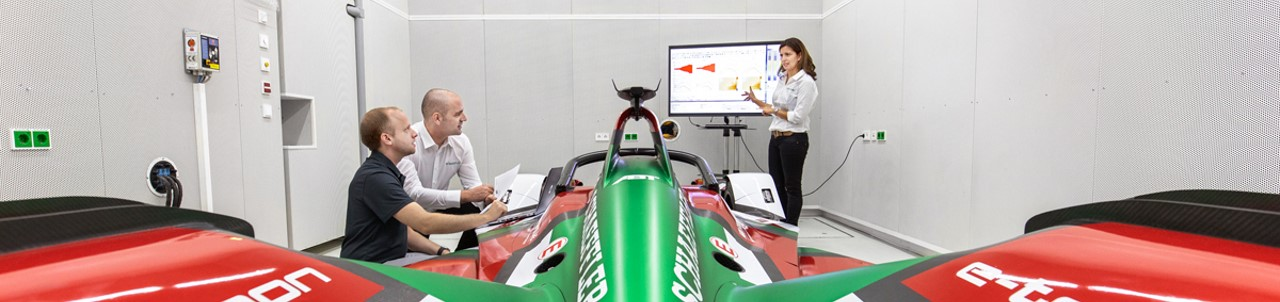
\includegraphics[width=16cm]{images/cover_sample.jpg}\\
	\vspace*{24mm}	für das 05. und 06. Theoriesemester (T3\_3101)\\
	\vspace*{3mm}		\langartikelstudiengang{} \langstudiengang{} \textbf{\studiengang}\\
	\vspace*{3mm}		\langanderdh{} \dhbw\\
	\vspace*{7mm}	\langvon\\
	\vspace*{3mm}		{\large\textbf \autor}\\
	\vspace*{7mm}	\datumAbgabe\\
\end{center}

\vfill

\flushleft
\begin{spacing}{1.2}
\begin{tabbing}
		mmmmmmmmmmmmmmmmmmmmmmmm              \= \kill
		\textbf{\langdbbearbeitungszeit} \> \zeitraum\\
		\textbf{\langdbmatriknr, \langdbkurs} \> \matrikelnr, \kurs\\
		\textbf{\langdbfirma} \> \firma\\
								\> \firmenort\\
		\textbf{\langdbgutachter}              \>  \gutachter\\
		\textbf{Kooperation}               \>  CURE Mannheim e.V.; Team Suspension\\
		\>  Coblitzallee 1-9, 68163 Mannheim\\
%		\> Team Suspension\\
		
\end{tabbing}
\end{spacing}
% \vspace{1cm}

\vspace{1cm}
\restoregeometry
\end{titlepage}